
%----------------------------------------------------------------------------------------
%	PACKAGES AND DOCUMENT CONFIGURATIONS
%----------------------------------------------------------------------------------------

\documentclass{article}

\usepackage[version=3]{mhchem} % Package for chemical equation typesetting
\usepackage{siunitx} % Provides the \SI{}{} and \si{} command for typesetting SI units
\usepackage{graphicx} % Required for the inclusion of images
\usepackage{natbib} % Required to change bibliography style to APA
\usepackage{amsmath} % Required for some math elements 
\usepackage{german}
\usepackage{float}
\restylefloat{figure}
\usepackage[utf8]{inputenc}
\setlength\parindent{0pt} % Removes all indentation from paragraphs
\renewcommand{\labelenumi}{\alph{enumi}.} % Make numbering in the enumerate environment by letter rather than number (e.g. section 6)

%\usepackage{times} % Uncomment to use the Times New Roman font

%----------------------------------------------------------------------------------------
%	DOCUMENT INFORMATION
%----------------------------------------------------------------------------------------

\title{Physiklabor \\ Laborbericht \\ Drehmoment und Drall} % Title

\author{Daniel \textsc{Hediger} \\ Lucien \textsc{Egloff}} % Author name



\date{\today} % Date for the report

\begin{document}

\maketitle % Insert the title, author and date

\begin{center}
\begin{tabular}{l r}
Ausführungsdatum: & September 28, 2016 \\ % Date the experiment was performed
Dozent: & Dr.Ackermann \\% Instructor/supervisor
Version:& 2.0
\end{tabular}


\end{center}

\newpage
\tableofcontents 

%----------------------------------------------------------------------------------------
%	SECTION 1
%----------------------------------------------------------------------------------------
\newpage
\section{Aufgabe 1}


Das Trägheitsmoment eines Rades soll durch das anhängen eines Gewichtes bestimmt werden.

\subsection{Grundlagen}

Das Gewicht wird durch die Erdbeschleunigung nach unten gezogen, und durch das Seil wird das Rad beschleunigt. Durch diese Beziehung kann die Winkelbeschleunigung und die Trägheit berechnet werden.

\subsection{Versuchsaufbau}
\begin{figure}[h]
\center

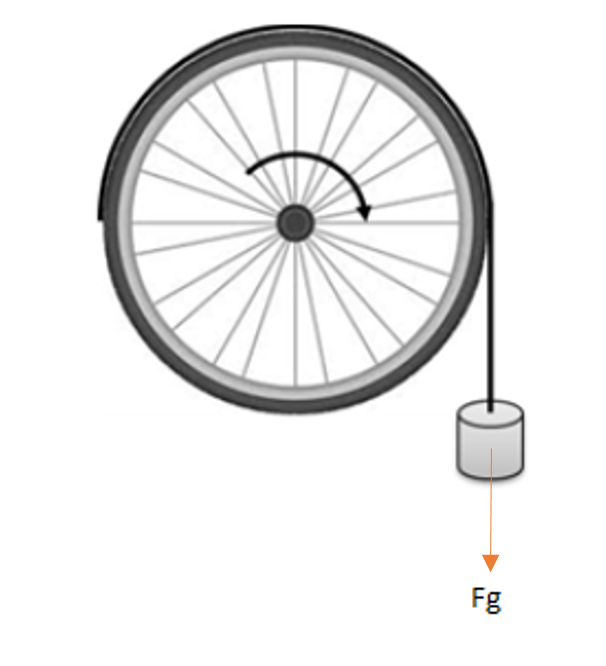
\includegraphics[scale=0.3]{Wheel.pdf} 
\caption{Fahrradrad mit angehängten Gewicht.}
\
\end{figure}

\subsection{Berechnungen}
Energieerhaltung des Systems.\begin{equation}
E_{rot}+E_{kin}=E_{pot}  \Rightarrow\frac{1}{2}*I*\omega^2+\frac{1}{2}*m*v^2=m*g*h
\end{equation}

Das ganze nach dem Trägheitsmoment umgestellt.
\begin{equation}
I=\frac{-m*(v^2-2g*h)}{\omega^2}
\end{equation}

Das fehlende $\omega$ wurde nun Experimentell bestimmt.


\begin{table}[H]
\center
    \begin{tabular}{|l|l|l|l|}
        \hline
        
  
        Durchgang & RPM$\cdot$2 $\ast$ $ \quad $[$\frac{1}{60s}$ ]   & $\omega \quad $[$\frac{rad}{s}$] & I $\quad [kg\cdot m^2]$ \\ \hline
        1         & 114.3 & 11.97 & 0.076 \\ 
        2         & 131   & 13.72 & 0.055 \\ 
        3         & 118   & 12.36 & 0.071 \\ 
        4         & 117   & 12.25 & 0.072 \\ 
        5         & 121   & 12.67 & 0.066 \\ 
        6         & 116   & 12.15 & 0.073 \\ 
        7         & 117.6 & 12.31 & 0.071 \\ 
        8         & 126.2 & 13.22 & 0.060 \\ 
        9         & 119   & 12.46 & 0.069 \\ \hline
        			\textbf{Mittelwert}&\textbf{120.01}&\textbf{12.57}&\textbf{0.068}\\
        \hline
  
    \end{tabular}
    \caption{Gemessene Grössen und daraus folgenden Berechnungen.}
      $\ast$  Für bessere Genauigkeit wurde RPM immer nach $\pi$ gemessen

\end{table}
\subsection{Schussfolgerung}

Ähnlich wie schon rechnerisch bestimmt, erhält man ungefähr das gleiche Trägheitsmoment.Mit einer Standartabweichung von nur $67*10^-4$ kann man davon ausgehen das die gemessen Grössen genügen aussagekräftig sind .Gewisse Abweichungen entstehen durch Messfehler und Reibungen am Rad.\newpage


\section{Aufgabe 2}
Das eigene Trägheitsmoment soll Experimentell aufgrund der Drehimpulserhaltung bestimmt werden.     
\subsection{Grundlagen}
Durch die Gegebenheit der Drehzahl des Rades und dessen Trägheitsmoment, kann anhand der eigenen
Drehzahl nach dem verändern der Drehachse, das Trägheitsmoment des gesamten 
Mensch-Hocker-Rad-Systems genähert werden.

\subsection{Versuchsaufbau}
\begin{figure}[h]
\center

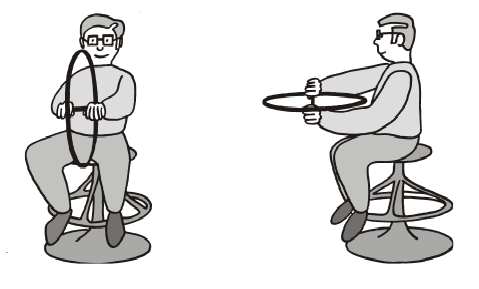
\includegraphics[scale=0.5]{Drehschemmel.pdf} 
\caption{Person mit drehendem Fahrradrad}
\

\end{figure}
\newpage
\subsection{Berechnungen}
Mit der Formel:
\begin{equation}
I_{Person}=\frac{I_{Rad}\cdot n_{Rad}\cdot T_{Stuhl}}{30}-(I_{Rad}+m_{Rad}\cdot d^2)
\end{equation}
können folgende Werte berechnet werden:
\begin{table}[H]
   \center
    \begin{tabular}{|l|l|l|l|}
        \hline
     
        Durchgang & $n_{Rad[1/min]}$ & $T_{Stuhl}[sek]$ & $I_{Person}\quad [kg\cdot m^2]$ \\ \hline
        1         & 1080         & 2.31    & 5.09      \\ 
        2         & 1080         & 2.26    & 4.96       \\ 
        3         & 1080         & 2.27    & 4.98        \\ 
        4         & 1100         & 34.1    & 3.79        \\ 
        5         & 1100         & 28.3    & 4.71        \\ 
        6         & 1100         & 30      & 4.40        \\ 
        7         & 1100         & 29.27   & 4.53        \\ 
        8         & 900          & 30.46   & 3.40        \\ 
        9         & 900          & 31.25   & 3.30        \\ 
        10        & 900          & 30.93   & 3.34        \\ \hline
        	\textbf{Mittelwert}&&&\textbf{4.25}\\
        \hline
    \end{tabular}
    \caption{Tabelle der Gemessen Grössen mit einer Standarbweichung des Mittelertes von 0.72$ kg\cdot m^2$ aus den Versuchen.}
\end{table}

\subsection{Schlussfolgerung}

Diverse Ungenauigkeiten, wie zum Beispiel die genaue Sitzposition der Person oder fehlende Angaben über das Trägheitsmoment des Stuhls, führten bei diesem Versuch dazu, dass das Resultat etwas weit ab von den Erwartungen(siehe Anhang)ausfiel. Man müsste bei der Berechnung im vornherein sicherlich noch die Position der Arme beachten, um das Trägheitsmoment korrekt bestimmen zu können.
\newpage
\section{Aufgabe 3}

Ein rotierender Kreisel wird durch das anhängen eines Gewichtes zum Präzessieren gebracht. Daraus lässt sich das Trägheitsmoment berechnen. 
\subsection{Grundlagen}
Durch das Anhängen eines Gewichts an den Kreisel, wirkt auf diesen ein Drehmoment, welches eine 
Präzession auslöst. Die Präzessionsfrequenz sagt aus wie viele Präzessionsperioden in einer Sekunde 
durchlaufen werden. Die Präazessionsperiode ist die Zeit, welche der Kreisel benötigt um eine Drehung um 2$\pi$ auszuführen.
\subsection{Gemessene Grössen}
Ein  Gewicht von 100g wurde in einem abstand von 70mm zum Zentrum angebracht.


\begin{table}[H]
   \center
    \begin{tabular}{|l|l|l|}
        \hline
        Durchgang & Drehzahl$[\frac{1}{60s}]$ & T $[sek]$    \\ \hline
        1         & 4500     & 51.58  \\ 
        2         & 1100     & 14.66 \\ 
        3         & 2200     & 26.53 \\ 
        4         & 6200     & 59.54 \\ 
        5         & 5200     & 43.04 \\ 
        6         & 5000     & 53.07\\ 
        7         & 2530     & 25.18  \\ \hline
        \textbf{Mittelwert}&\textbf{3818}&\textbf{39.17}\\
        \hline
    \end{tabular}
    \caption{Tabelle mit gemessenen Grössen aus dem Versuch.}
\end{table}
\textbf{Berechnungen}
$T_{Praezession} = 39.17s$ ,
$n_{Kreisel=3818min^-1}$ ,
$r=70mm$\\
\begin{equation}
W_{Kreisel}=2 \cdot \pi	\cdot \frac{n_{Kreisel}}{60}=2 \cdot \frac{3818}{60}= \underline{199.91}rad
\end{equation}

\begin{equation}
M=r \cdot m \cdot g \cdot = 0.07 \cdot 0.1 \cdot 9.81 = \underline{0.0687Nm}
\end{equation}
\begin{equation}
 I_{Kreisel}= \frac{M \cdot T_p}{\omega \cdot 2\pi}= \frac{0.0687 \cdot 39.17}{199.91 \cdot 2\pi}= \underline{\underline{0.0020kgm^2}}
\end{equation}

\subsection{Schlussfolgerung}
Das im Dossier angegebene Trägheitsmoment des Kreisels beträgt 0.0014 kgm2. Unser im Versuch
ermitteltes Trägheitsmoment liegt als nur 0.0007 neben dem ebenfalls mittels Versuch ermittelten
Trägheitsmoment. Diese Abweichung rührt hauptsächlich aus der Ungenauigkeit der Zeitmessung, da
diese von Hand mittels Stoppuhr erfolgte.
\section{Aufgabe 4}
Der Drallsatz soll durch das einwirken einer horizontalen Kraft bestimmt werden.
\subsection{Grundlagen}
Der Kreisel wird beschleunigt und anschliessend mit einer Horizontalen Kraft belastet. Dadurch beginnt er sich zu drehen, und die Zeit die er für $90^\circ$ benötigt wird gemessen. Anschliessend werden wir mit Hilfe des Drallsatzes, der gemessenen Werte und des Trägheitsmoments, die Kraft welche wir aufwendeten berechnen und auf Übereinstimmung überprüfen.

\subsection{Berechnungen}
\begin{table}[H]
   \center
    \begin{tabular}{|l|l|l|l|}
        \hline
           Durchgang & Drehzahl$[\frac{1}{60s}]$ & F $[Nm]$&T $[sek]$     \\ \hline
        1         & 1400    & 0.5 & 13.60  \\ 
        2         & 1450    & 0.5 & 14.25  \\ 
        3         & 1400    & 0.5 & 11.49\\ 
        4         & 3300     & 0.5 & 24.00 \\ 
        5         & 2850     & 0.5 & 20.52 \\
        \hline
        \textbf{Mittelwert}&\textbf{2080}&\textbf{0.5}&\textbf{16.6}\\ \hline
    \end{tabular}
    \caption{Tabelle mit gemessenen Grössen aus dem Versuch}
\end{table}
\begin{equation}
M_z=F \cdot r = 0.5 \cdot 0.07 = \underline{0.035Nm}
\end{equation}
\begin{equation}
\omega_K= 2\pi \cdot\frac{n_k}{60} = 2080 \cdot \frac{\pi}{30} = \underline{217.8s^-1}
\end{equation}
\begin{equation}
\Delta Lz=M_z*T=0.035Nm \cdot 16.6s = \underline{\underline{0.581 [\frac{Kg\cdot m^2}{s}]}} 
\end{equation}
Für den Drallsatz $M = \frac{dl}{dt}$ gilt im Fall einer $90^\circ$ Verkippung DL=L.
Zum Vergleich:
\begin{equation}
L_k = I_k \cdot\omega_k = 0.002 \cdot  217.8 = \underline{0.435}
\end{equation}



\subsection{Schlussfolgerung}
Abweichung der Werte bei $90^\circ$ beträgt 25 Prozent.
Die Abweichung hat in diesem Versuch mehrere Gründe:\\\\
\textbf{1)} Die Kraft F (5 N) und damit das Moment waren nicht während der ganzen Rotationsdauer
konstant. Dies hat ein Schwanken der Präzessionsgeschwindigkeit zur Folge und so indirekt
Einfluss auf die gemessene Zeit.\\
\textbf{2)} Die Zeit wurde von Hand mittels Stoppuhr gemessen\\
\textbf{3)} Die Drehzahl des Kreisels hat sich während der Messung durch Reibungsverluste und Luftwiederstand
verringert.
\newpage
\section{Aufgabe 5}

\subsection{Grundlagen}
Der Versuch diente zur Bestimmung des Bremsmomentes am Velorad und am Kreisel.
Hierzu wurde das Rad und der Kreisel in Rotation versetzt und die Drehzahl in bestimmten Zeitintervallen
gemessen. Durch die Abnahme der Drehzahl konnte das Bremsmoment mit dem Trägheitsmoment
berechnet werden.
\subsection{Gemessene Grössen}

\begin{figure}[H]
\includegraphics[scale=0.5]{Diagramm.pdf} 
\caption{Gemessene Grössen und Trendverlauf.}
\end{figure}
Aus diesen Werten werden folgende Trendlininen berechnet:\\
Trend Rad : \hspace{2cm}$-4.3t+397 $\\
Trend Kreisel : \hspace{1.58cm}$-11t+2828$

Durch die Ableitung nach der Zeit dieser Werte erhalten wir die Winkelbeschleunigung $\alpha$.\\
Ersichtlich wird dabei das der Kreisel doppelt so schnell bremst wie das Rad.\\\\
Das bremsende Drehmoment ergibt sich aus: 
\begin{equation}
M=I\cdot \alpha
\end{equation}
\begin{equation}
M_{Kreisel} = I_{Kreisel}\cdot \alpha = 0.0021kgm^2 \cdot (-11)\frac{1}{s^2} = \hspace{0.4cm}-0.0231Nm\\
\end{equation}
\begin{equation}
M_{Rad} = I_{Rad}\cdot \alpha= 0.07kgm^2 \cdot (-4.3)\frac{1}{s^2}  =  -0.301Nm
\end{equation}
\subsection{Berechnungen}
Das Bremsmoment sowie die Winkelgeschwindigkeit sind in den Messwerttabellen(Anhang 2) bei der dazugehörigen Drehzahl zu finden.

\begin{figure}[H]
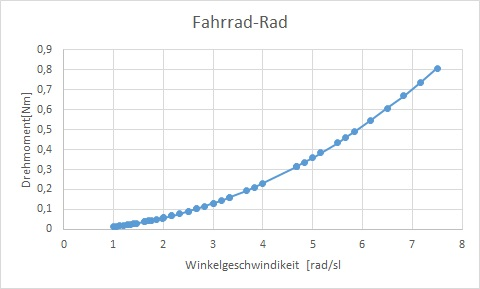
\includegraphics[scale=0.7]{Fahrradw.pdf} 
\caption{Gemessen Daten des Fahrradrades.}
\end{figure}
\begin{figure}[H]
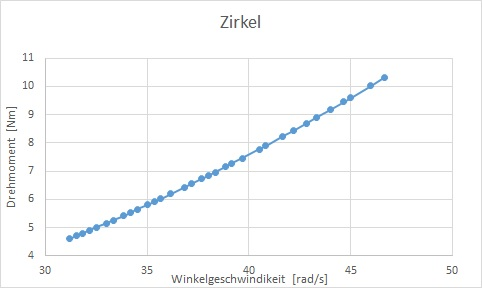
\includegraphics[scale=0.7]{Zirkelw.pdf} 
\caption{Gemessen Daten des Zirkels.}
\end{figure}



\subsection{Schlussfolgerung}
Die Messwerte sind mit Vorsicht zu geniessen, da die Drehzahlen von Hand in den Zeitintervallen
abgelesen wurden. 
Der Versuch mit dem Kreisel müsste viel länger dauern, sodass auch bei kleinen Winkelgeschwindigkeiten
Messwerte vorliegen.
Der Vergleich Kreisel Fahrrad zeigt, dass der Kreisel ähnliche Werte bei viel höheren Drehzahlen
erreicht. Der Grund dafür wird der grössere Luftwiderstand am Fahrrad durch Pneu und Speichen
sein.
\newpage
\section{Anhang}

\begin{figure}[H]

\includegraphics[scale=0.4]{Berechnung.pdf} 
\end{figure} 

\begin{figure}[H]

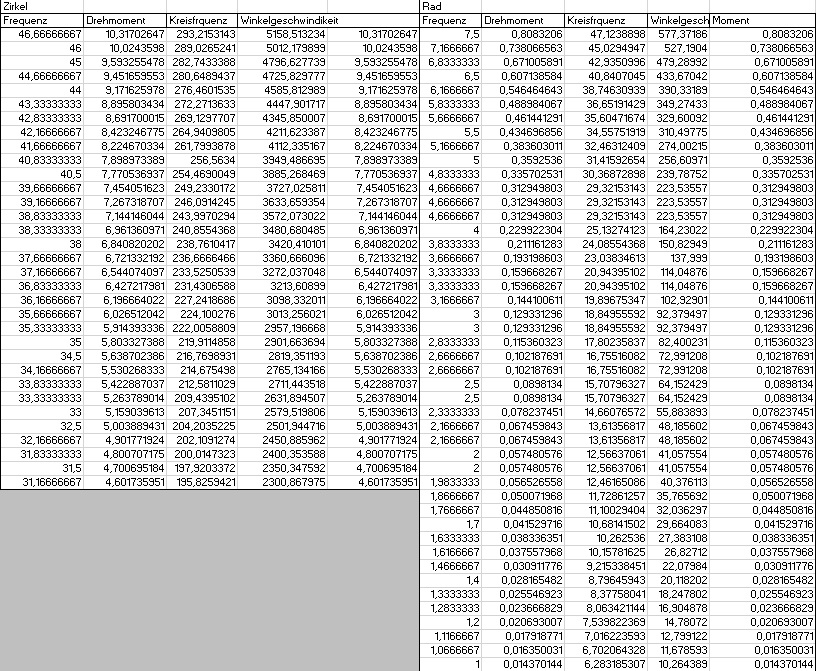
\includegraphics[scale=0.6]{Tabelle.pdf} 
\end{figure} 
\end{document}